% Final report (English translation of informe-final.tex, public version)
% Build from reporte/: latexmk -pdf report-final-en.tex
\documentclass[11pt,letterpaper]{article}

\usepackage[T1]{fontenc}
\usepackage[utf8]{inputenc}
\usepackage{lmodern}
\usepackage[english]{babel}
\usepackage[margin=2.5cm]{geometry}
\usepackage{microtype}
\usepackage{amsmath,amssymb}
\usepackage{booktabs,tabularx,array}
\usepackage{enumitem}
\usepackage[table]{xcolor}
\usepackage{graphicx}
\graphicspath{{../figuras/}{figuras/}}
\usepackage{caption}
\usepackage{float}
\usepackage{titlesec}
\usepackage{fancyhdr}
\usepackage[round,authoryear]{natbib}
\usepackage[hidelinks]{hyperref}

\definecolor{tinta}{HTML}{1F3A5F}
\definecolor{acento}{HTML}{B5432A}
\definecolor{suave}{HTML}{EEF2F6}

\titleformat{\section}{\large\bfseries\color{tinta}}{\thesection.}{0.6em}{}
\titleformat{\subsection}{\normalsize\bfseries\color{tinta}}{\thesubsection}{0.6em}{}
\setlist{itemsep=2pt,topsep=4pt}
\captionsetup{font=small,labelfont=bf}
\renewcommand{\arraystretch}{1.22}
\newcolumntype{L}{>{\raggedright\arraybackslash}X}
\newcolumntype{R}{>{\raggedleft\arraybackslash}X}

\pagestyle{fancy}
\fancyhf{}
\lhead{\small Final report}
\rhead{\small Sensory propagation in the \emph{Drosophila} connectome}
\cfoot{\small\thepage}
\renewcommand{\headrulewidth}{0.4pt}

\hypersetup{pdftitle={Final report: sensory propagation in the Drosophila connectome},
            pdfauthor={Atlahua Quiahuitl Martínez Obregón}}

\begin{document}

% ---------------------------------------------------------------- header
\begin{center}
{\small Universidad Autónoma Metropolitana, Azcapotzalco · Computer Engineering\par}
\vspace{0.5cm}
{\Large\bfseries\color{tinta} Final report\par}
\vspace{0.15cm}
{\large Sensory propagation in the \emph{Drosophila} connectome: from the brain to the nerve cord\par}
\vspace{0.4cm}
{\normalsize Atlahua Quiahuitl Martínez Obregón\par}
{\small Period: 17--21 November 2026 · Submitted Saturday, 21 November 2026\par}
{\footnotesize\itshape English translation of the Spanish report (\texttt{informe-final.pdf}). Figure labels are in Spanish; captions explain them.\par}
\vspace{0.2cm}
{\color{tinta}\rule{\linewidth}{0.6pt}}
\end{center}

\begin{abstract}
\noindent This report measures in how many steps information from each sensory modality reaches every neuron of the fruit fly and its motor neurons, using the probabilistic traversal model of \citet{schlegel2021} on two public connectomes: the FlyWire v783 brain and the BANC v888 brain and nerve cord. An independent, vectorized implementation, validated against \texttt{navis}, reproduces the layers published by \citet{dorkenwald2024} for all 13 modalities (Spearman 0.971 to 0.996), but only with the whole brain, no synapse threshold and a 15-step cap. The criteria for the BANC were fixed before opening its data. The order of layers per cell type is preserved between the two flies (Spearman 0.964 to 0.978): H2 holds. In the full central nervous system, each leg's mechanosensory neurons reach that leg's motor neurons 1.5 to 2.1 steps sooner than the closest head modality, about 3 layers beyond what 10 degree-preserving random graphs give. But the fixed criterion required 2 steps in all three legs and only the hind leg reaches it: H3 is not met as stated. The synapse threshold changes the layers (Spearman 0.88); the step cap does not. Code, figures and results are in a public repository (v0.2).
\end{abstract}

% ---------------------------------------------------------------- 1
\section{Question, hypotheses and final status}

\begin{quote}
\emph{In how many layers of the traversal model does information from each sensory modality reach the leg and wing motor neurons, when the full path through the brain and the nerve cord is followed?}
\end{quote}

\begin{table}[H]
\centering
\small
\begin{tabularx}{\linewidth}{@{}p{2.9cm}Lp{3.2cm}@{}}
\toprule
\textbf{Question} & \textbf{Criterion} & \textbf{Result} \\
\midrule
H1. Replication & Spearman $\rho \ge 0.9$ per modality against the published layers & \textbf{Met} (13 of 13) \\
H2. Two flies & Median $\rho$ per cell type $\ge 0.7$ and at least 3 of 4 modalities $\ge 0.7$ & \textbf{Met} (4 of 4) \\
H3. Cord shortcut & In each leg, its mechanosensory neurons reach its motor neurons at least 2 steps sooner than the best head modality, with a 95\,\% CI excluding 0 and larger than in 10 random graphs; in all three legs & \textbf{Not met} (T3 only) \\
P4. Sensitivity & No hypothesis: median and range of $\rho$ between configurations & Threshold matters; cap does not \\
\bottomrule
\end{tabularx}
\caption{Hypotheses of the protocol and results. The criteria for H2, H3 and the control were written in the plan on 20 November 2026, 23:40, before opening the BANC data, and were not changed.}
\end{table}

\noindent The five phases of the plan were completed between 17 and 21 November. Public repository: \url{https://github.com/Quiwitl/fly-sensory-layers}, version 0.2.

% ---------------------------------------------------------------- 2
\section{Data}

\begin{itemize}
  \item \textbf{FlyWire v783.} Connections from Zenodo (record 10676866) and annotations from \citet{schlegel2024}. 139{,}262 neurons, 15{,}091{,}983 connected pairs without threshold (54.5 million synapses) and 2{,}700{,}513 pairs with 5 or more synapses. The thresholded figures match the published ones.
  \item \textbf{Published layers.} One table per modality with the mean layer of each neuron over 10{,}000 runs \citep{rangos2024}.
  \item \textbf{BANC v888.} From Harvard Dataverse \citep{bancdata}: the \texttt{simple\_v2} edge list (11{,}752{,}828 pairs without threshold, the one used by \citealp{bates2026}) and the annotations (188{,}508 rows). Glia, non-neuronal elements and rows without a superclass are removed. H2 keeps 122{,}575 neurons and 7.72 million pairs (brain: \texttt{central\_brain} and \texttt{optic\_lobe}); H3 keeps 146{,}769 neurons and 10.65 million pairs (whole central nervous system).
  \item \textbf{Seeds and targets in the BANC.} Olfactory (3{,}007), head gustatory (380), Johnston's organ (1{,}193), visual projection (7{,}316), and front, middle and hind leg mechanosensory neurons (1{,}322, 1{,}302 and 1{,}539). Targets: leg motor neurons T1 (139), T2 (126), T3 (126) and wing motor neurons (64).
\end{itemize}

\begin{figure}[H]
\centering
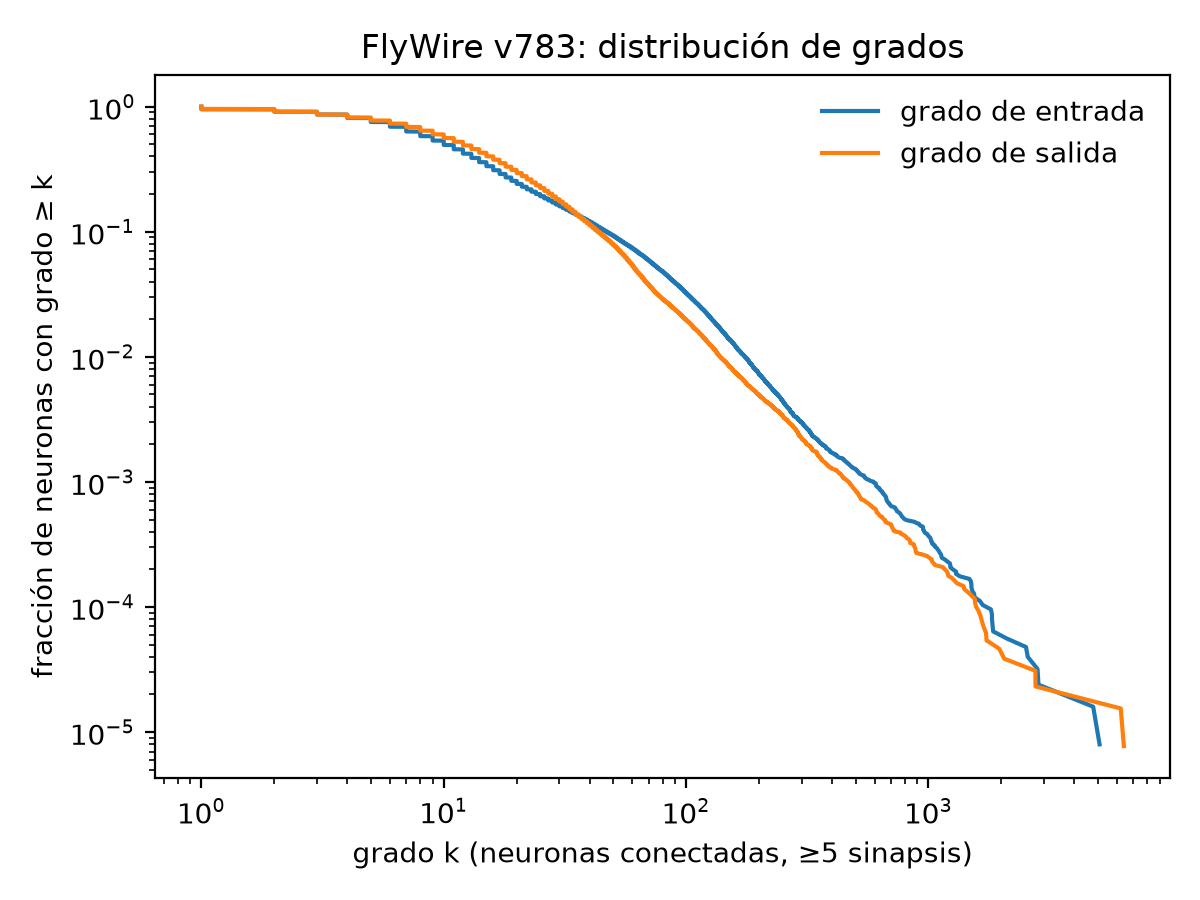
\includegraphics[width=0.5\linewidth]{01_grados.png}
\caption{Degree distribution of FlyWire v783 (5 or more synapses): in-degree and out-degree.}
\end{figure}

% ---------------------------------------------------------------- 3
\section{Method}

\subsection{Traversal model}

Seed neurons are layer 1. At each step, every edge $i\to j$ from an already-traversed neuron to one that is not succeeds with probability
\[
p_{ij}=\min\!\left(1,\ \frac{A_{ij}}{0.3}\right), \qquad A_{ij}=\frac{W_{ij}}{\sum_k W_{kj}},
\]
where $W$ is the synapse count and $A$ the fraction of $j$'s inputs that come from $i$. Neuron $j$ is traversed if any of its edges succeeds, and its layer is that step. A neuron that fails is drawn again at the next step. A run ends when no candidate edges remain or at the step cap. The layer of each neuron is the mean over runs. This is what \texttt{TraversalModel} in \texttt{navis} does \citep{navis}.

\subsection{Implementation}

\begin{enumerate}
  \item \textbf{One draw per neuron.} Instead of drawing each edge, each neuron is drawn once with $P_j = 1-\prod_i(1-p_{ij})$, which has the same distribution. The product is computed as $1-\exp\!\big(\sum_i \log(1-p_{ij})\big)$: a sparse matrix product with the vector of traversed neurons.
  \item \textbf{Batches of runs.} Each run is a column of a dense matrix, so one step of 100 runs is a single sparse-times-dense product.
  \item \textbf{Stopping rule.} In FlyWire, batches of 100 runs are added until the mean layer changes by less than 0.01 in 99\,\% of the neurons (at least 5 batches). In the BANC, 1{,}000 runs per modality are always done.
  \item \textbf{GPU.} \texttt{recorrido\_gpu.py} does the same with CuPy \citep{cupy}: the matrices are copied to the card and each step is a cuSPARSE product. The stopping rule is the same.
\end{enumerate}

\subsection{Validation}

\begin{itemize}
  \item \textbf{Tests.} 9 tests on synthetic graphs (normalization, chain, exact 30\,\% input, direction, reproducibility, speed, edge rule and retry) and property-based tests.
  \item \textbf{Against \texttt{navis}.} On a 1{,}610-neuron subgraph, the mean difference in non-seed neurons is 0.001 layers.
  \item \textbf{GPU against CPU.} In FlyWire, same configuration and three modalities: $r \ge 0.999$, bias of 0.017 layers or less and the same neurons reached. In the BANC, the same random graph on both engines: $r \ge 0.994$ and the H3 measure equal to two decimals.
\end{itemize}

\subsection{Analysis}

\begin{itemize}
  \item \textbf{H1.} Spearman between own and published layer per modality, seeds excluded.
  \item \textbf{H2.} Mean layer per cell type in FlyWire and in the BANC brain, matched by \texttt{fafb\_cell\_type}; Spearman per head modality, 15-step cap.
  \item \textbf{H3.} Median layer of each leg's motor neurons from each modality, 30-step cap (15 also reported). Difference = layer from the closest head modality $-$ layer from the leg's mechanosensory neurons; 95\,\% CI by bootstrap over motor neurons (1{,}000 resamples).
  \item \textbf{Control.} 10 random graphs that keep every neuron's in- and out-degree, by edge swapping \citep{maslov2002}: 10 rounds, about 51.6 million swaps per graph, all 10.65 million pairs kept. The H3 traversal is repeated on each graph.
  \item \textbf{P4.} Spearman of the mean layer per neuron between FlyWire runs that only change the threshold (5 vs.\ 1 synapse) or the cap (15 vs.\ 30 steps). As a noise reference, two runs of the same configuration are compared (CPU vs.\ GPU).
\end{itemize}

% ---------------------------------------------------------------- 4
\section{Results}

\subsection{H1: replication in FlyWire}

The first comparison did not meet H1, and the cause was the graph, not the model. The Methods of \citet{dorkenwald2024} describe the central brain with a 5-synapse threshold, but their layers only come out with another graph:

\begin{table}[H]
\centering
\small
\begin{tabularx}{\linewidth}{@{}LXX@{}}
\toprule
\textbf{Graph} & \textbf{Spearman (13 modalities)} & \textbf{Layer difference} \\
\midrule
Central brain, $\ge 5$ synapses, 30 steps & 0.65 -- 0.95 & up to 1.4 layers \\
Whole brain, $\ge 5$ synapses, 15 steps & 0.82 -- 0.95 & 0.06 to 1.2 layers later \\
\textbf{Whole brain, no threshold, 15 steps} & \textbf{0.971 -- 0.996} & \textbf{0.05 -- 0.15 layers} \\
\bottomrule
\end{tabularx}
\caption{Replication by graph, 1{,}000 runs per modality. Only the last configuration meets H1.}
\end{table}

\noindent Three clues led to that configuration: the published table has about 124 thousand neurons, more than the central brain (62 thousand); with the whole brain, own layers came out later precisely in distant neurons, as if paths were missing; and the maximum published layer is exactly 15, the default cap in \texttt{navis}. Per modality, Spearman ranges from 0.971 (taste peg) to 0.996 (photoreceptors) and the mean layer difference from 0.05 to 0.15. Olfactory neurons reach the olfactory Kenyon cells first and visual projection neurons the visual Kenyon cells, as reported.

\begin{figure}[tbp]
\centering
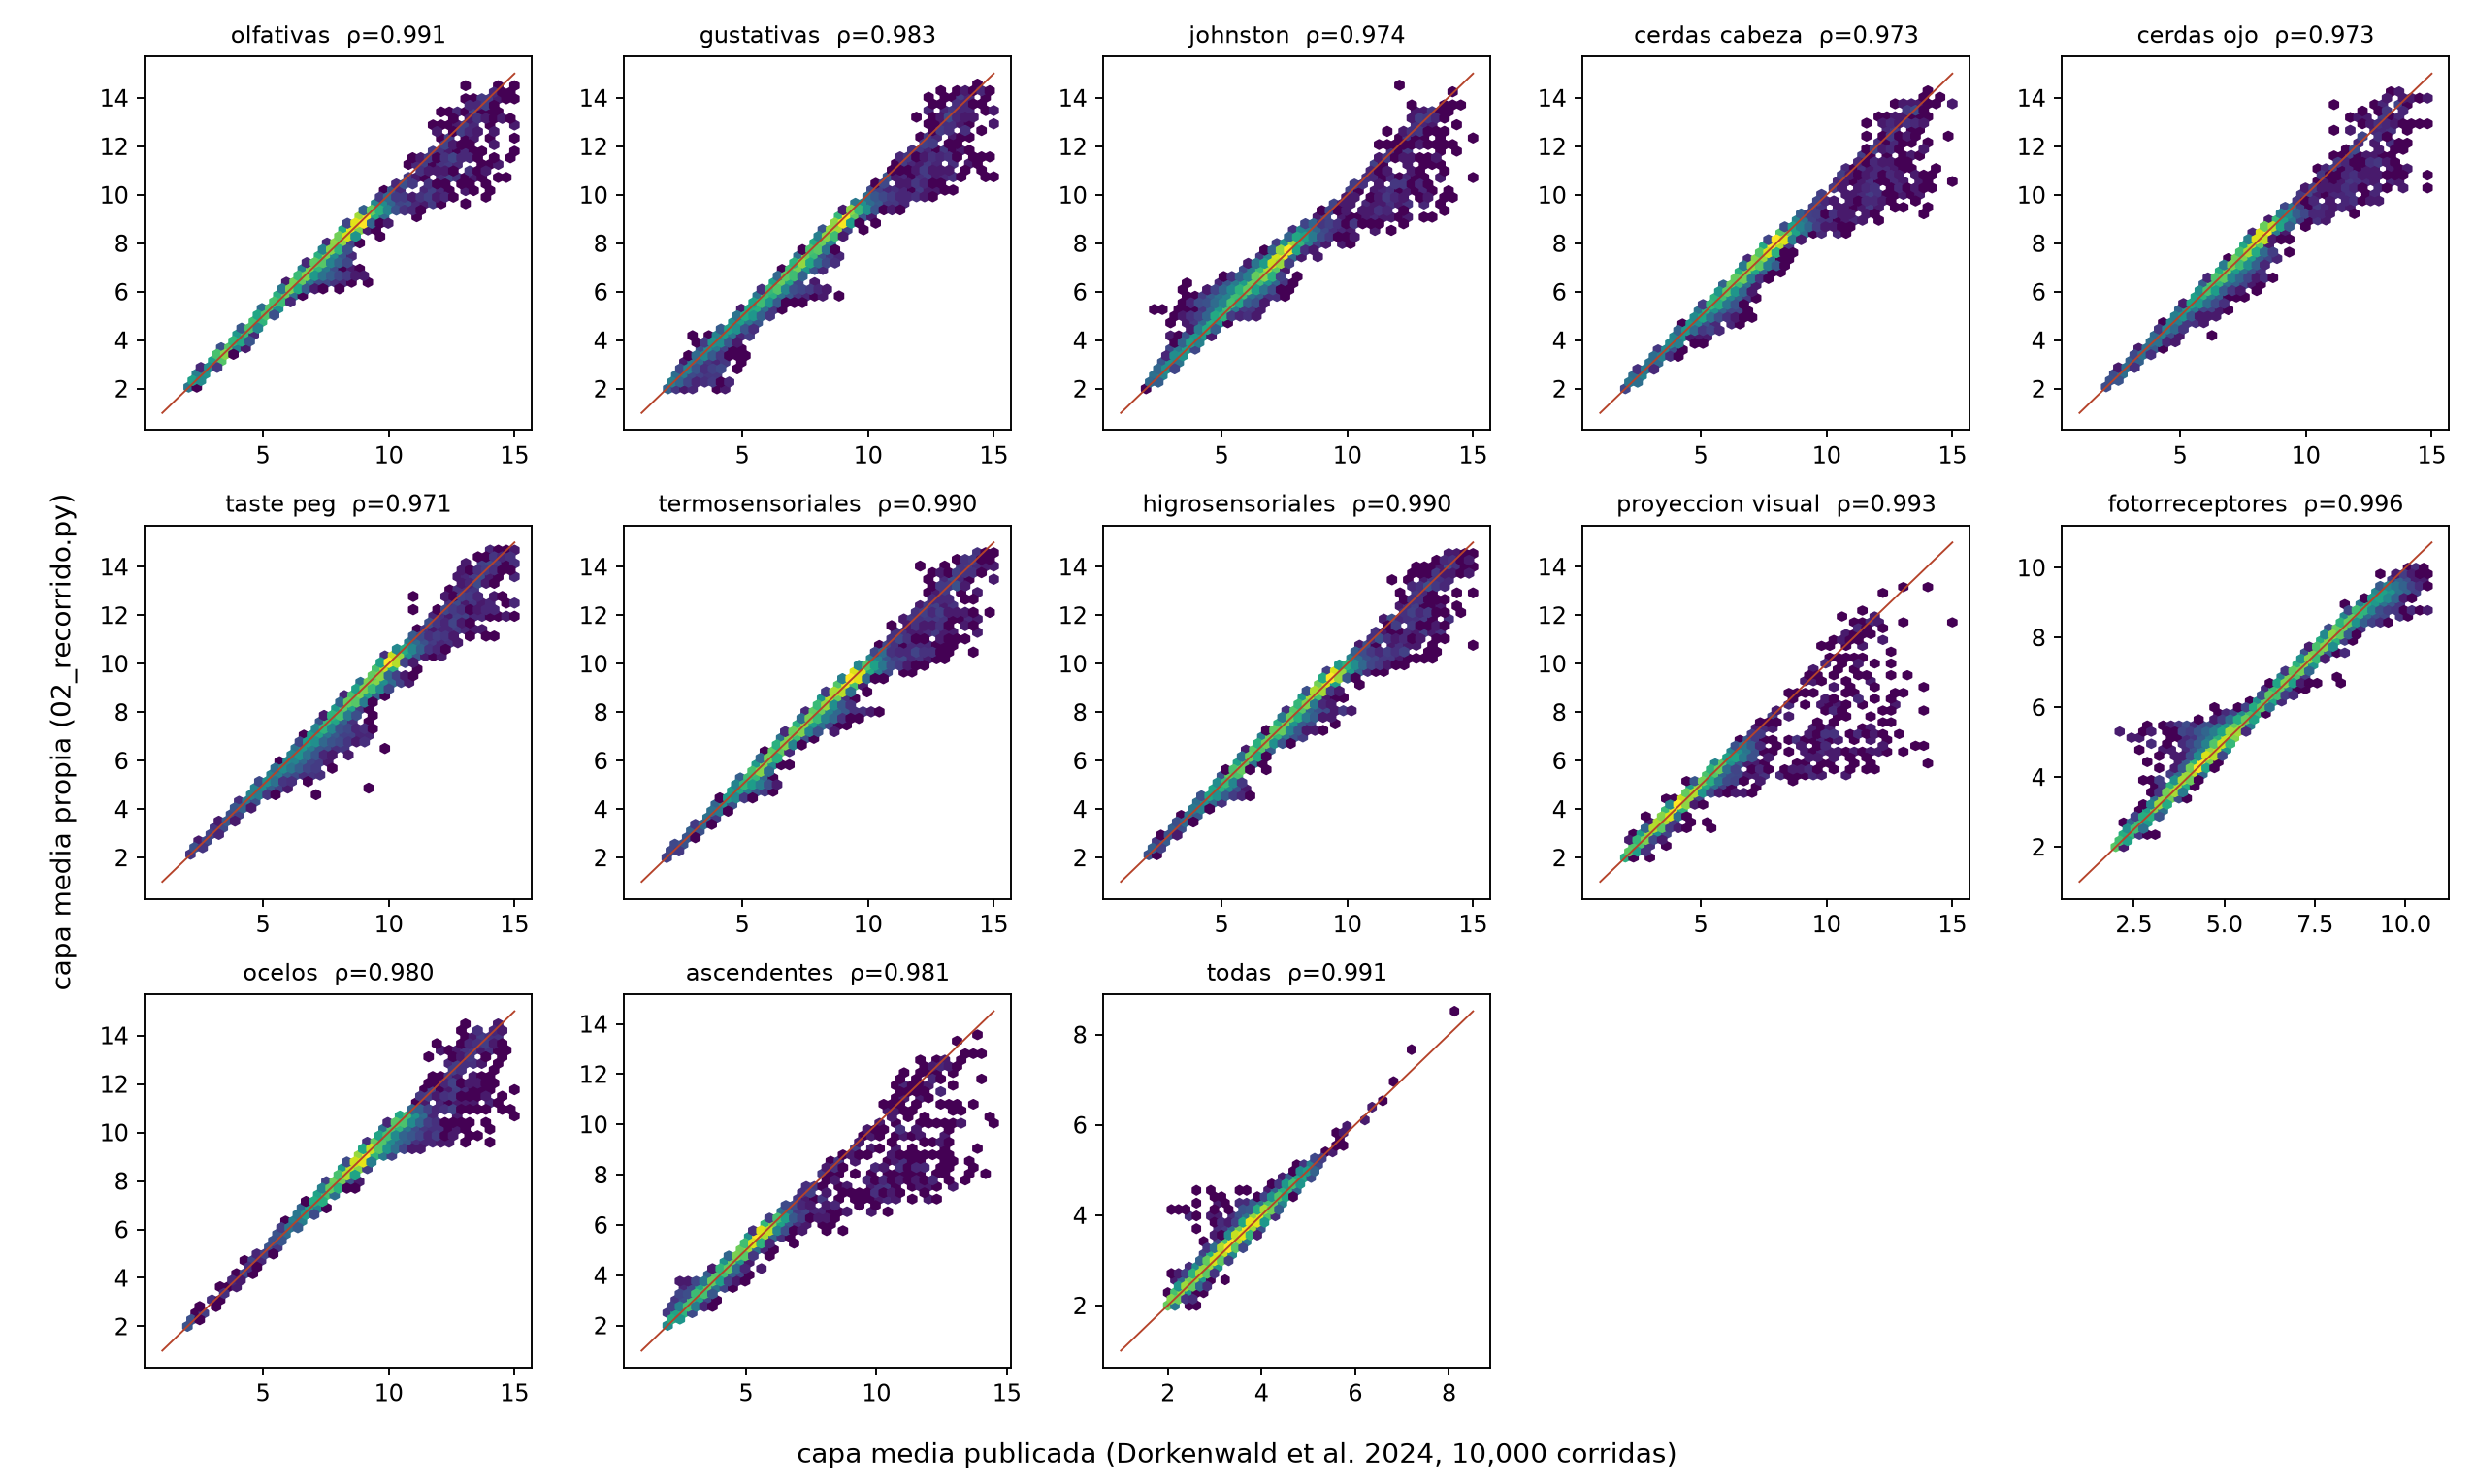
\includegraphics[width=0.92\linewidth]{03_propio_vs_publicado_completo_p15_u1.png}
\caption{Own mean layer (vertical) against published mean layer (horizontal) per modality (whole brain, no threshold, 15 steps). The red line is equality.}
\end{figure}

\subsection{H2: the same order in two flies}

\begin{table}[H]
\centering
\small
\begin{tabularx}{0.85\linewidth}{@{}LRR@{}}
\toprule
\textbf{Modality} & \textbf{All types (7{,}528)} & \textbf{Types with $\ge 5$ neurons (1{,}507)} \\
\midrule
Olfactory & 0.972 & 0.984 \\
Gustatory & 0.971 & 0.975 \\
Johnston's organ & 0.964 & 0.972 \\
Visual projection & 0.978 & 0.985 \\
\midrule
Median & \textbf{0.971} & \textbf{0.980} \\
\bottomrule
\end{tabularx}
\caption{Spearman of the mean layer per cell type between FlyWire and the BANC brain. H2 holds in all 4 modalities.}
\end{table}

\noindent Without seeds or optic lobe, 6{,}859 types remain, with Spearman from 0.967 to 0.975, and the median difference BANC $-$ FlyWire ranges from $-0.21$ to $+0.33$ layers. As the protocol expected, types with more neurons agree better.

\begin{figure}[H]
\centering
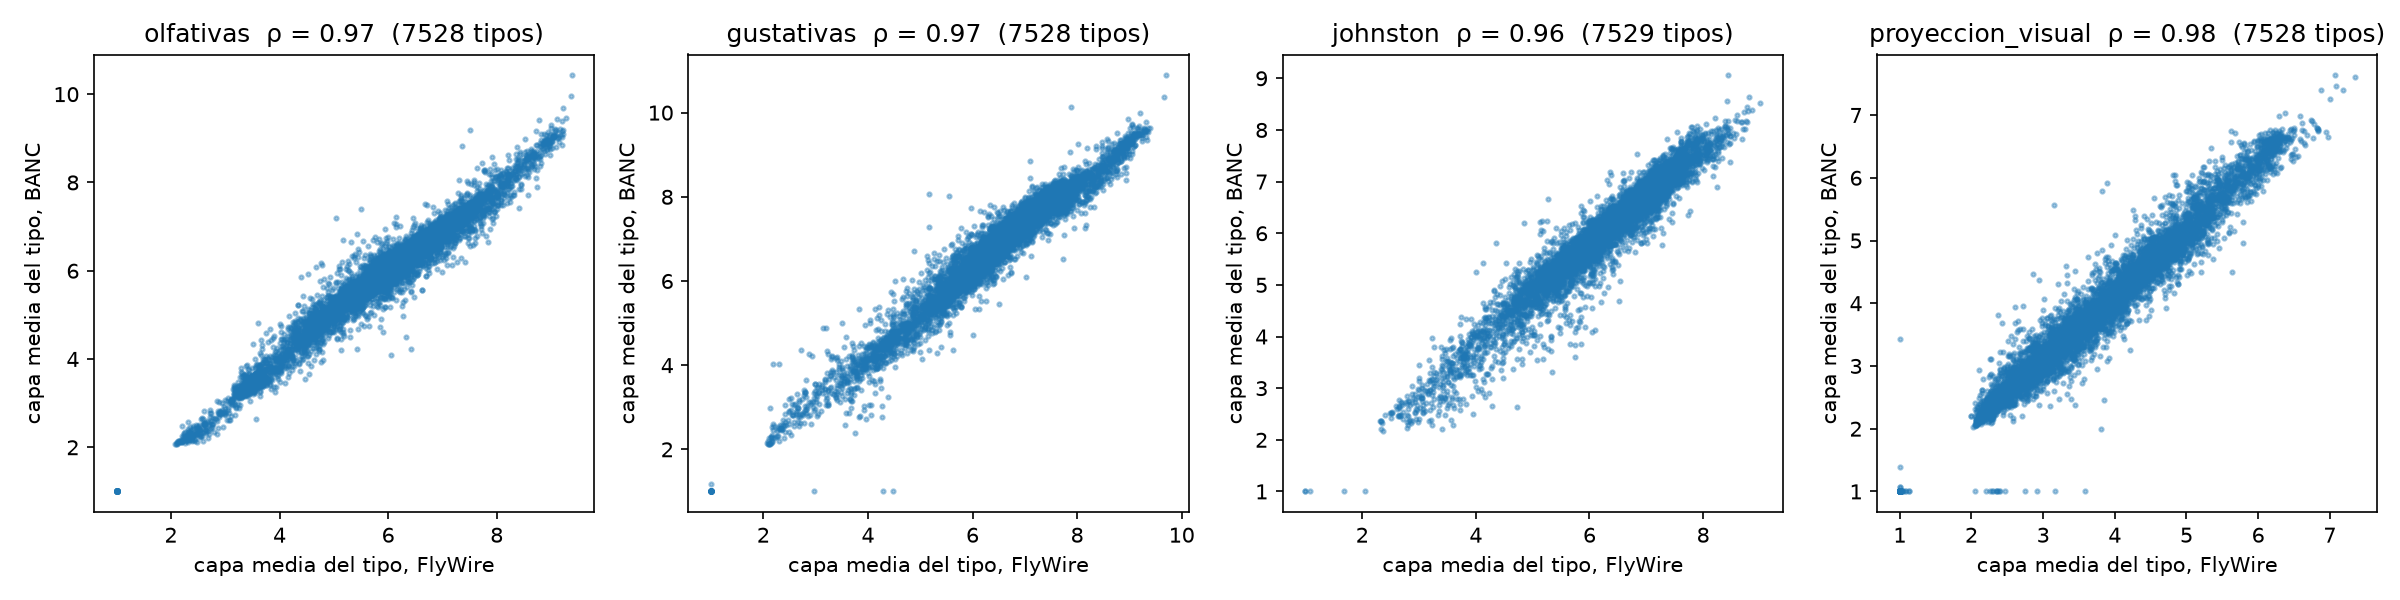
\includegraphics[width=\linewidth]{05_h2_tipos.png}
\caption{Mean layer per cell type in FlyWire (horizontal axis) and in the BANC (vertical axis), per modality (\emph{olfativas}: olfactory, \emph{gustativas}: gustatory, \emph{johnston}: Johnston's organ, \emph{proyeccion\_visual}: visual projection).}
\end{figure}

\subsection{H3: the leg shortcut}

\begin{table}[H]
\centering
\small
\begin{tabularx}{\linewidth}{@{}LRRRR@{}}
\toprule
\textbf{From} & \textbf{T1 leg MNs} & \textbf{T2 leg MNs} & \textbf{T3 leg MNs} & \textbf{Wing MNs} \\
\midrule
T1 mechanosensory & \textbf{3.95} & 5.38 & 5.67 & 5.94 \\
T2 mechanosensory & 5.40 & \textbf{3.68} & 5.30 & 5.61 \\
T3 mechanosensory & 5.69 & 5.34 & \textbf{3.56} & 5.65 \\
Visual projection & 5.43 & 5.47 & 5.64 & 4.96 \\
Johnston's organ & 6.35 & 6.44 & 6.62 & 5.84 \\
Gustatory & 6.74 & 7.08 & 7.19 & 7.30 \\
Olfactory & 7.47 & 7.76 & 7.97 & 7.75 \\
\bottomrule
\end{tabularx}
\caption{Median layer of the motor neurons (MNs) of each segment from each modality, in the full BANC central nervous system (30-step cap; identical with 15, because all are reached in 100\,\% of runs).}
\end{table}

\noindent The diagonal is clear: each leg's mechanosensory neurons reach the motor neurons of their own segment sooner than those of the other legs. Among head modalities, the closest to the legs is always visual projection, and the farthest is olfaction.

\begin{table}[H]
\centering
\small
\begin{tabularx}{\linewidth}{@{}p{1.2cm}XXp{2.2cm}p{2.6cm}@{}}
\toprule
\textbf{Leg} & \textbf{Real graph (95\,\% CI)} & \textbf{10 random graphs (range)} & \textbf{Larger than all 10?} & \textbf{Shortcut by the criterion?} \\
\midrule
T1 & 1.48 (1.42 -- 1.53) & $-1.55$ to $-1.49$ & yes & no ($<2$ steps) \\
T2 & 1.79 (1.74 -- 1.84) & $-1.26$ to $-1.22$ & yes & no ($<2$ steps) \\
T3 & 2.08 (2.00 -- 2.12) & $-1.34$ to $-1.30$ & yes & \textbf{yes} \\
\bottomrule
\end{tabularx}
\caption{Difference = layer from visual projection $-$ layer from the leg's mechanosensory neurons. Identical with a 15-step cap.}
\end{table}

\noindent In the random graphs the sign flips: the mechanosensory neurons end up 1.2 to 1.5 steps \emph{farther} from their leg's motor neurons than visual projection, and the 10 graphs barely differ from each other (range of 0.06 steps or less). So the proximity in the real graph, about 3 layers beyond chance, is not explained by the degree distribution: it is specific wiring. But the fixed criterion required at least 2 steps in all three legs, and T1 and T2 fall short. \textbf{H3 is not met as stated.}

\begin{figure}[H]
\centering
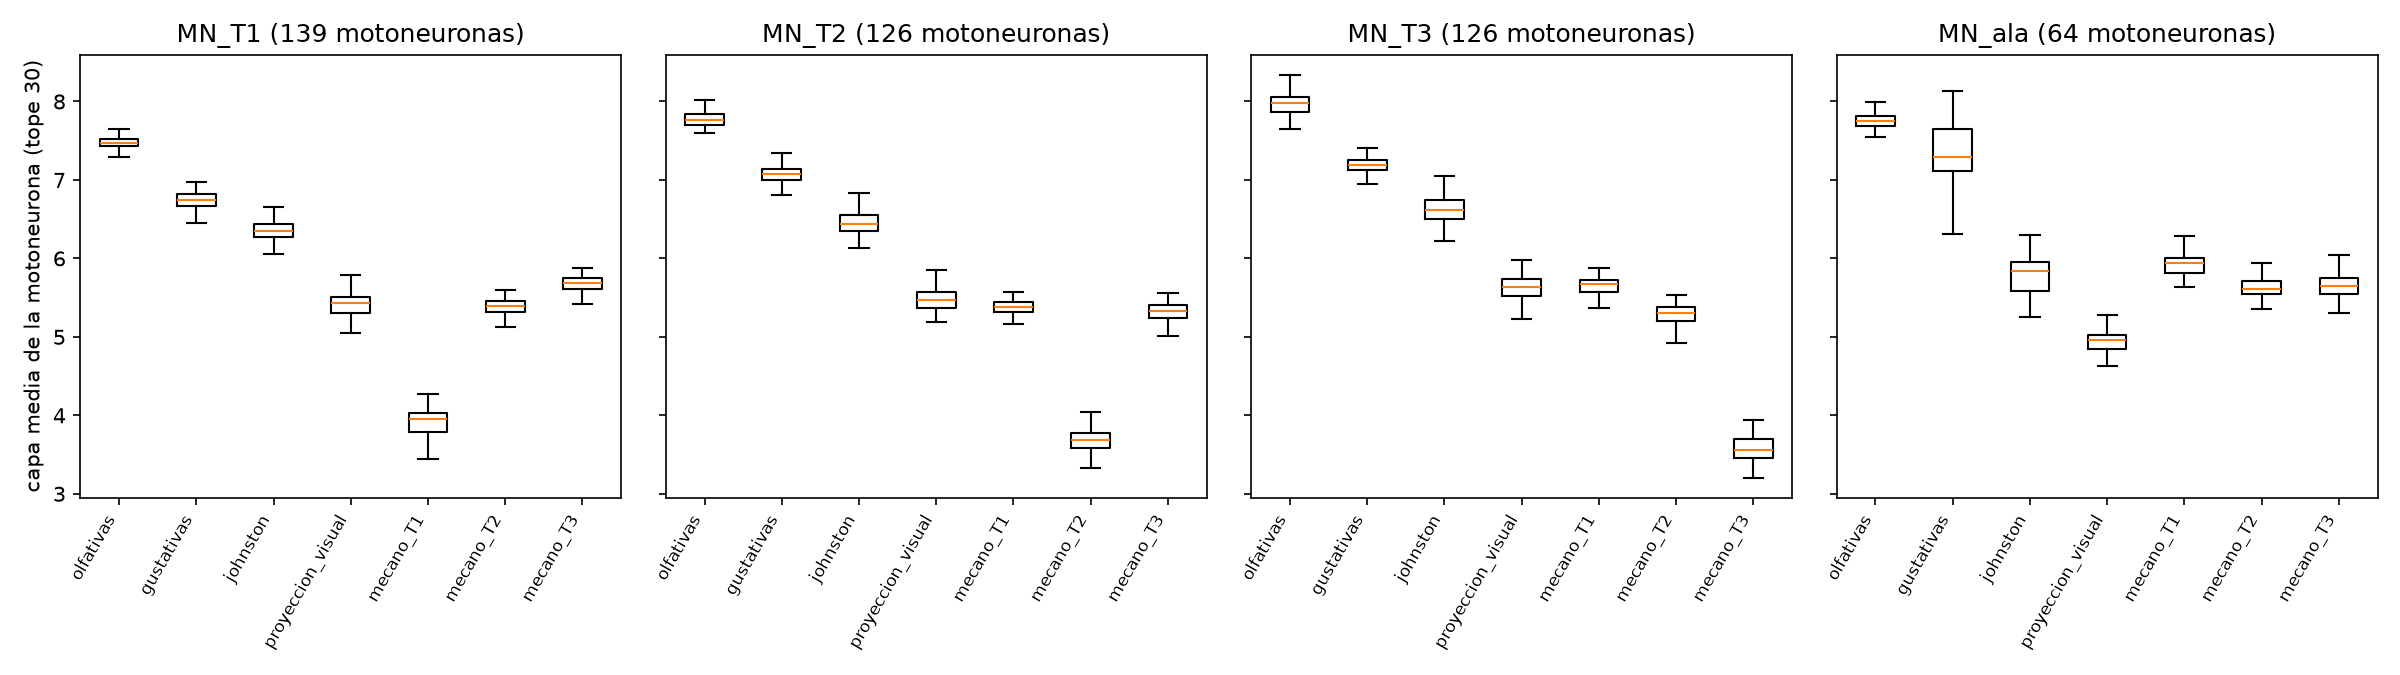
\includegraphics[width=\linewidth]{05_h3_motoneuronas.png}
\caption{Mean layer of the motor neurons of each segment (T1, T2, T3 legs and wing) from each modality (30-step cap).}
\end{figure}

\subsection{P4: sensitivity to threshold and cap}

\begin{table}[H]
\centering
\small
\begin{tabularx}{\linewidth}{@{}Lp{1.7cm}p{2.5cm}L@{}}
\toprule
\textbf{Comparison} & \textbf{Median $\rho$} & \textbf{Range} & \textbf{Layer shift} \\
\midrule
Threshold: 5 vs.\ 1 synapse (15-step cap) & 0.880 & 0.837 -- 0.958 & without threshold, 0.07 to 1.25 layers earlier; about 12 thousand more neurons per modality \\
Cap: 15 vs.\ 30 steps (no threshold) & 0.9985 & 0.9975 -- 0.9998 & 0.02 layers or less; no new neurons \\
Noise: same configuration, CPU vs.\ GPU & 0.9971 & 0.9955 -- 0.9997 & 0.017 layers or less \\
\bottomrule
\end{tabularx}
\caption{Spearman of the mean layer per neuron in 12 FlyWire modalities, seeds excluded. The three threshold and cap runs were done on the GPU with the same stopping rule (1{,}800 to 2{,}900 runs per modality).}
\end{table}

\noindent The effect of the cap is within noise. The effect of the threshold is not: connections with fewer than 5 synapses bring arrival forward and add neurons. The most affected modalities are the ocelli and the eye bristles.

\begin{figure}[H]
\centering
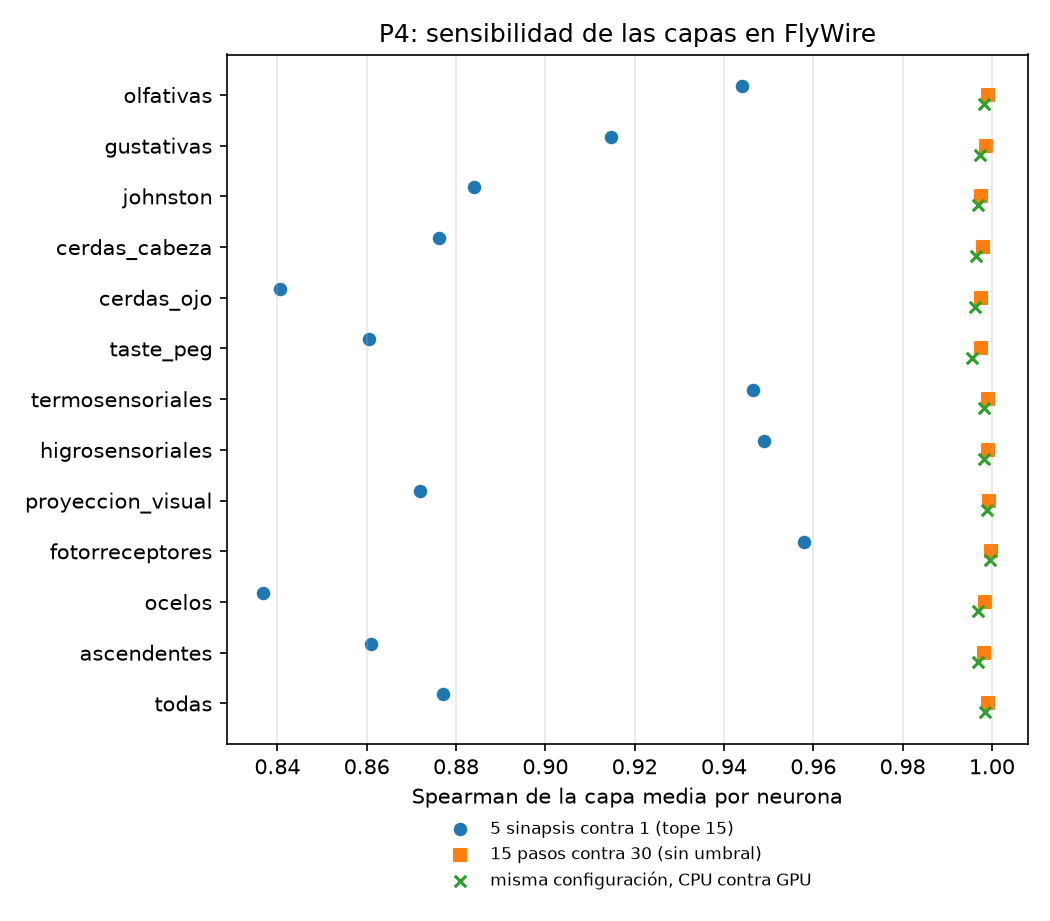
\includegraphics[width=0.75\linewidth]{06_sensibilidad.png}
\caption{Spearman per modality in each P4 comparison: threshold (5 vs.\ 1 synapse), cap (15 vs.\ 30 steps) and noise (CPU vs.\ GPU).}
\end{figure}

% ---------------------------------------------------------------- 5
\section{Discussion}

\begin{enumerate}
  \item \textbf{Weak connections count.} H1 and P4 say the same thing from two sides: the published layers are only reproduced without a threshold, and removing the threshold shifts layers by up to 1.25 steps. Traversal layers from two studies can only be compared if they use the same threshold, and it should always be reported with the layers. The step cap, in contrast, does not matter from 15 on.
  \item \textbf{The layer order belongs to the cell type, not the individual.} With two flies reconstructed by different teams, the order holds with $\rho \approx 0.97$. This supports using the traversal layer as a property of each cell type.
  \item \textbf{The shortcut exists, but it is smaller than proposed.} All three legs have a path to their motor neurons shorter than the head's and far above chance. What fails is the size: 2 steps was a reasonable threshold, but it was chosen without a precedent that fixed it. The result is reported as it came out; moving the threshold to 1.5 after seeing the data would make H3 pass, and that is why it is not done.
\end{enumerate}

\subsection{Limitations}

\begin{itemize}
  \item \textbf{H2 includes the optic lobe.} Almost all visual projection neurons in the BANC are annotated in \texttt{optic\_lobe}; with \texttt{central\_brain} only, that modality disappears. The literal version (central brain only) remains in the code as an option.
  \item \textbf{Input fraction within each subgraph.} In H2 the fraction $A_{ij}$ is computed without the inputs that come from the cord, so it is not identical to the full-CNS one.
  \item \textbf{Runs.} The BANC was run with 1{,}000 runs per modality, without a convergence rule (change in the last batch of 0.025 to 0.038 layers in 99\,\% of the neurons). The H3 intervals are narrow, so the verdict does not change, but individual layers carry that noise.
  \item \textbf{Seeds.} BANC gustatory seeds are head neurons only; leg gustatory neurons are left out so as not to mix them with mechanosensory ones.
  \item \textbf{Unexplained difference.} Between 15 and 17 thousand neurons get an own layer in FlyWire and do not appear in the published table. It does not affect the Spearman values, because only neurons present in both are compared, but the reason is unknown.
  \item \textbf{A single model.} Everything depends on the traversal model and its 0.3 threshold. Other closeness measures, such as the influence score of \citet{bates2026}, were not compared, because they already made that comparison.
\end{itemize}

% ---------------------------------------------------------------- 6
\section{Changes from the protocol}

\begin{table}[H]
\centering
\small
\begin{tabularx}{\linewidth}{@{}p{3.4cm}LL@{}}
\toprule
\textbf{What} & \textbf{Before} & \textbf{Now and why} \\
\midrule
H1 graph & Central brain, 5 synapses & Whole brain, no threshold, 15 steps: it is what reproduces the published layers \\
Model rule & Per neuron & Per edge, with retry: it is what \texttt{navis} does \\
P4 & Traversal vs.\ BANC influence & Sensitivity to threshold and cap: \citet{bates2026} already compared their influence with traversal \\
H2 region & Brain without cord & \texttt{central\_brain} and \texttt{optic\_lobe}, to keep visual projection \\
Runs & 10{,}000 per modality & 1{,}000 in H1 and the BANC; in P4, until convergence (1{,}800 to 2{,}900) \\
Compute & CPU & Optional GPU, validated against the CPU; the control and P4 ran on the GPU \\
\bottomrule
\end{tabularx}
\caption{Deviations from the protocol and their justification. None touches the criteria for H2, H3 or the control.}
\end{table}

% ---------------------------------------------------------------- 7
\section{Reproducibility}

Everything is reproduced from the repository with \texttt{uv}, which installs each script's dependencies:

\noindent\begin{minipage}{\linewidth}
{\small
\begin{verbatim}
uv run 00_descargar.py          # FlyWire, annotations, published layers and BANC (MD5)
uv run pruebas_recorrido.py     # model tests
uv run 02_validar_navis.py      # against navis
uv run 02_recorrido.py --alcance completo --umbral-sinapsis 1 \
       --max-pasos 15 --max-corridas 1000
uv run 03_validar_publicado.py _completo_p15_u1          # H1
uv run 04_banc.py --h2 ; uv run 04_banc.py --h3            # H2 and H3
uv run 04_azar_lote.py          # the 10 random graphs (--gpu for the GPU)
uv run 05_evaluar_banc.py       # H2, H3 and the control
python 02_recorrido.py ... --gpu --etiqueta _gpu          # three P4 runs
uv run 06_sensibilidad.py       # P4
\end{verbatim}
}
\end{minipage}
\medskip

\noindent Times on a 16-thread laptop with an 8~GB RTX 5050: a BANC random graph takes about 31 minutes on the CPU (4 processes) and about 6 on the GPU; a full FlyWire run, 18 to 35 minutes on the CPU and 2 to 16 on the GPU. The data are not redistributed: FlyWire is CC BY-NC 4.0; the published layers and the BANC, CC BY 4.0. The code is MIT-licensed.

% ---------------------------------------------------------------- 8
\section{Self-assessment}

The protocol was assessed with the AAC\&U \emph{Inquiry and Analysis} rubric \citep{aacu2009} and the CCH research-project rubric \citep{cchunam}, and left for this report the criteria that needed results.

\begin{table}[H]
\centering
\small
\rowcolors{2}{suave}{white}
\begin{tabularx}{\linewidth}{@{}p{3.1cm}Lc@{}}
\toprule
\textbf{Criterion} & \textbf{Evidence in this report} & \textbf{Level} \\
\midrule
Design & Criteria for H2, H3 and the control fixed before seeing the data; random-graph control; model validated at three levels & 4 \\
Analysis & Results organized by hypothesis, with intervals, control and a noise reference & 4 \\
Conclusions & They follow from the findings; H3 is reported as not met even though the shortcut exists & 4 \\
Limitations & Six concrete limitations, with their effect on the results & 3--4 \\
Writing and citation & Clear and concise; \texttt{apalike} style, similar to but not identical with APA & 3 \\
\bottomrule
\end{tabularx}
\caption{Self-assessment of the criteria that depended on the results.}
\end{table}

% ---------------------------------------------------------------- 9
\section{Conclusions}

I consider that the project answered its question. Sensory information reaches the leg motor neurons in about 3.5 to 4 steps from the mechanosensory neurons of the same leg, in about 5.4 to 5.6 from vision and in almost 8 from olfaction. The order of layers in the brain is stable between two flies, and the leg shortcut is real: it is far above chance. What did not hold is the size I myself set for that shortcut, and I prefer to report it that way rather than move the criterion.

What I learned most is not in the hypotheses. Replicating a published result forced me to find decisions the paper does not state (the whole graph, no threshold, a 15-step cap), and those decisions turned out to be exactly what moves the layers most. I also learned to fix the criteria before seeing the data: without that, the H3 result would have been easy to present as a success.

Still open: why 15 to 17 thousand neurons appear in the own layers but not in the published ones, and whether the leg shortcut changes in another fly with a nerve cord once another complete connectome exists.

\bibliographystyle{apalike}
\bibliography{referencias-en}

\end{document}
